\chapter{Структура порождающей модели матрицы кросс-спектральной плотноти. 
         Подпространство протечки сигнала.} \label{chapt1}

\section{Постановка задачи оценки фазовой синхронности по неинвазивным измерениям} \label{sect1_1}

% Мы можем сделать \textbf{жирный текст} и \textit{курсив}.

Рассмотрим типичную постановку эксперимента по изучению некоторых
нейрофизиологических явлений с помощью ЭЭГ/МЭГ.
Предположим, что было сделано $К$ записей результатов тестов гомогенной электрофизической
активности объекта $\alpha$ продолжительностью $\Delta t$ с помощью устройства, имеющего m сенсоров.
Более того, допустим, что информация об анатомии мозга объекта α известна (этого можно достичь,
используя стандартную модель мозга или снимок МРТ мозга объекта).
Последнее допущение позволяет нам ввести пространство источников, представляющее собой сетку,
состоящую из n точек, аппроксимирующую поверхность мозга объекта (см.рис.1).
Решая так называемую прямую задачу [2], мы можем осуществить отображение точек пространства
источников n в m-мерное пространство сенсоров
(обычно $n >> m$, так как для качественной аппроксимации нам нужно намного
больше точек поверхности мозга, чем число сенсоров, которым мы располагаем)
с оператором отображения $\mathbf{G}$.
Оператор $\mathbf{G}$ решает уравнения Максвелла для точечных источников электромагнитной активности,
расположенных в каждом узле сетки, определяющей конфигурацию источников в пространстве,
и пока уравнения Максвелла остаются линейными, оператор $\mathbf{G}$ также является линейным \cite{Hamalainen1993}.
Мы также должны учесть влияние шума источники которого располагаются во внешней среде
и который принимается как белый шум.
Теперь мы можем записать порождающую модель измерений сенсорами

\begin{figure}
\centering
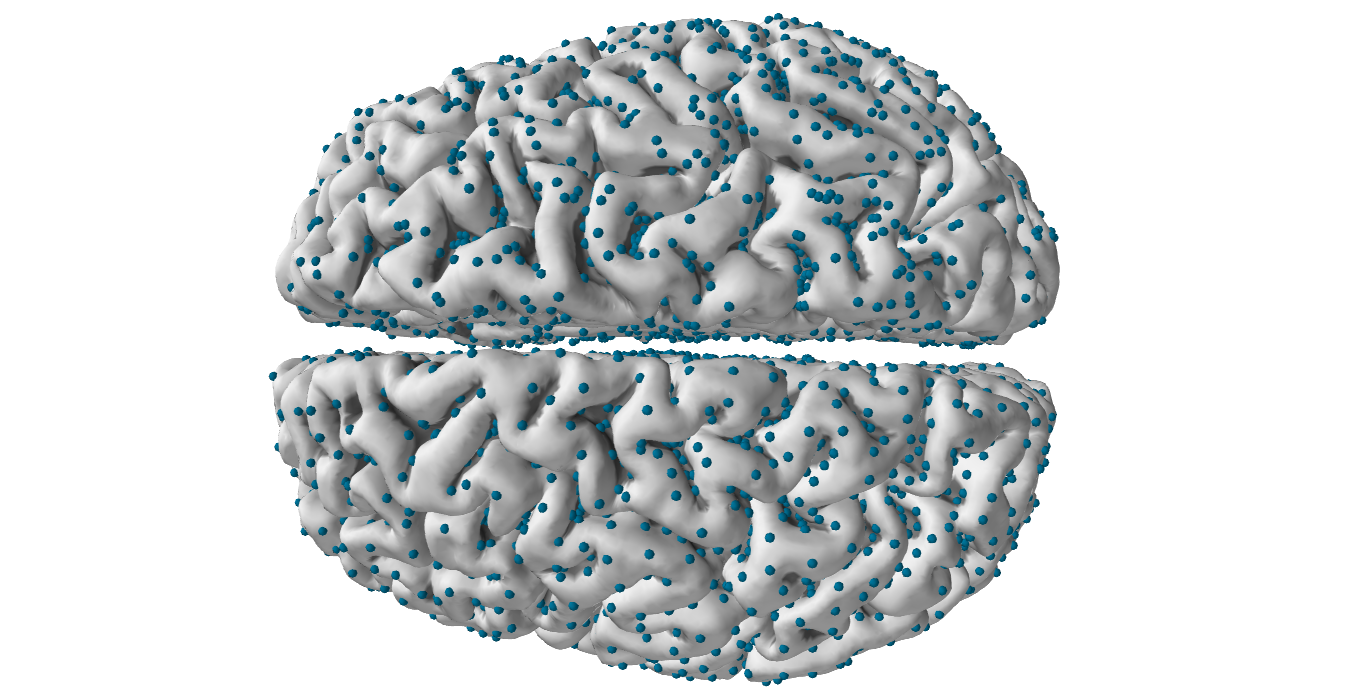
\includegraphics[scale=0.3]{../images/brain.png}
\caption{Пример сетки в пространстве источников,
          построенной на основе трехмерной анатомической модели}
\label{fig:src_space}
\end{figure}

\begin{equation}
    \mathbf{x}_k(t) = \mathbf{G} \cdot \mathbf{s}_k(t) + \mathbf{\omega}_k(t),
    \label{gm_ts}
\end{equation}
где $\mathbf{s}_k(t)$  вектор-столбец активаций источников размера $n \times 1$
$\mathbf{x}_k(t)$ вектор-столбец сигналов, снятых сенсорами,
размера $m \times 1$, $t$ --- время, $\mathbf{G}$ --- $m \times n$ матрица линейного отображения пространства источников в пространство сигналов.
Индекс $k$ обозначает номер эпохи.
Применим к (\ref{gm_ts}) частотное преобразование. Существует несколько способов произвести
эту операцию, например, --- вейвлет-преобразование или применение узкополосного фильтра
с задаваемыми резонансными частотами и последующим аналитическим представлением сигнала.
Мы не будем вдаваться в подробности теории частотно-временных преобразований;
для подробного математизированного изложения предмета см.
\cite{Oppenheim1998}, о  применении  частотно-временных преобращований к обработке
электрофизиологических данных можно прочитать в \cite{Freeman}.
Мы только упомянем, что вне зависимости от особенностей выбранного
метода образом частотно-временного преобразования матрицы $\mathbf{X}$ размера $m \times T$

будет комплексный тензор, каждый временной срез которого содержит в себе информацию
о фазовом и амплитудном спектре сигнала в каждый момент времени.
Чтобы упростить вывод, мы зафиксируем частоту и примем,
что соотношения справедливы для всех остальных частот преобразования. В итоге мы можем записать:

\begin{equation}
    \hat{\mathbf{x}}_{k,f_i}(t) = \mathbf{G} \cdot \hat{\mathbf{s}}_{k,f_i}(t) + \hat{\mathbf{\omega}}_{k,f_i}(t),
    \label{gm_timefreq}
\end{equation}
где $\hat{\mathbf{x}}, \hat{\mathbf{s}}, \hat{\mathbf{\omega}}$ --- комплекснозначные образы $\mathbf{x}, \mathbf{s}, \mathbf{\omega}$. Для простоты опустим индекс $f_i$ имея в виду, что все дальнейшие выкладки сделаны для одной фиксированной частоты: 

\begin{equation}
    \hat{\mathbf{x}}_k(t) = \mathbf{G} \cdot \hat{\mathbf{s}}_k(t) + \hat{\mathbf{\omega}}_k(t)
    \label{gm_timefreq_no_fi}
\end{equation}

Теперь, если мы для каждой эпохи умножим $\hat{\mathbf{x}}_k(t)$ на ее эрмитово сопряжение  и усредним результат, мы получим порождающую модель кросс-спектра на сенсорах:

\begin{gather}
           \langle{\hat{\mathbf{x     }}_k(t) \hat{\mathbf{x}}_k(t)^{\dag}} \rangle_{k=1}^K = 
           \langle{(\mathbf{G} \cdot\hat{\mathbf{s}}_k(t) + \hat{\mathbf{\omega}}_k(t))
                                       (\mathbf{G} \cdot\hat{\mathbf{s}}_k(t) + \hat{\mathbf{\omega}}_k(t))^{\dag}}\rangle_{k=1}^K=\nonumber\\
= \mathbf{G}  \cdot \langle{\hat{\mathbf{s     }}_k(t) \hat{\mathbf{s     }}_k(t)^{\dag}} \rangle_{k=1}^K \cdot \mathbf{G}^T + 
   \mathbf{G} \cdot \langle{\hat{\mathbf{s     }}_k(t) \hat{\mathbf{\omega}}_k(t)^{\dag}} \rangle_{k=1}^K + \nonumber\\
        +  \langle{\hat{\mathbf{\omega}}_k(t) \hat{\mathbf{s     }}_k(t)^{\dag}} \rangle_{k=1}^K \cdot \mathbf{G}^T +
           \langle{\hat{\mathbf{\omega}}_k(t) \hat{\mathbf{\omega}}_k(t)^{\dag}} \rangle_{k=1}^K, 
    \label{gm_cp_ini}
\end{gather}
\\
где оператор $\langle \cdot \rangle_{k=1}^K$ означает усреднение по эпохам. Так как шум предполагается белым, а сигнал на сенсорах $\hat{\mathbf{s}}_k$ и шум $\hat{\mathbf{\omega}}_k$ взаимно независимыми, можем заметить, что второй и третий члены уравнения (\ref{gm_cp_ini}) равны нулю, когда число эпох достаточно велико.
Также отметим, что
$\hat{\mathbf{x     }}_k(t) \hat{\mathbf{x     }}_k(t)^{\dag}$,
$\hat{\mathbf{s     }}_k(t) \hat{\mathbf{s     }}_k(t)^{\dag}$ и
$\hat{\mathbf{\omega}}_k(t) \hat{\mathbf{\omega}}_k(t)^{\dag}$
представляют собой внешние произведения комплексно-значных векторов на свои комплексные сопряжения,
и следовательно являются эрмитовыми матрицами, что означает,
что значения, находящиеся на их диагоналях, принадлежат области вещественных чисел.
Это свойство, очевидно, сохраняется и после усреднения.
Более того, раз элементы векторов являются комплексными числами, они могут быть представлены в виде
$\hat{\xi}(t) = r(t)\cdot e^{i\phi(t)}$, где $\phi(t)$ соответствует мгновенной фазе сигнала,
а $r(t)$ амплитуде. Следовательно,
$\langle \hat{\xi}_p \hat{\xi}_q^* \rangle = \langle r_p r_q e^{i\Delta\phi} \rangle$ или,
если для пояснения мы примем, что амплитуды и фазы по умолчанию независимы (справедливость последнего является предметом разногласий для электрофизиологических данных \cite{Lachaux1999}, \cite{imcoh}),
мы получим, что
$\langle \hat{\xi}_p \hat{\xi}_q^* \rangle = \langle r_p r_q \rangle \langle e^{i\Delta\phi} \rangle$
Из последнего соотношения можно сделать несколько выводов.
Во-первых, элементы матрицы кросс-спектра представляют собой степень стабильности
разности фаз $\Delta\phi$ по эпохам.
Если разность фаз достаточно равномерно распределена по всему возможному
интервалу принимаемых значений, то среднее $\langle e^{i\Delta\phi} \rangle$
приблизительно равно нулю.
С другой стороны, если разность фаз сохраняется от эпохи к эпохе,
результирующий коэффициент будет отличен от нуля,
что соответствует случаю установления коннективности между сигналами.
Во-вторых, если разность фаз мала,
элементы взаимного спектра могут быть близки к ненулевому вещественному числу.
Введем следующее обозначение для матрицы кросс-спектральной плотности: 

\begin{equation}
    \Cp{v} \stackrel{def}{=} \langle{\hat{\mathbf{v}}_k(t) \hat{\mathbf{v}}_k(t)^{\dag}}\rangle_{k=1}^K, \\
    \label{cp_def}
\end{equation} 
Используя определение (\ref{cp_def}) и опуская начальные условия, (\ref{gm_cp_ini})
перепишется в виде
\begin{equation}
    \Cp{x}(t) = \mathbf{G} \Cp{s}(t) \mathbf{G}^T + \Cp{\omega}(t)
    \label{gm_cp_matr}
\end{equation}

Теперь рассмотрим подробнее главную диагональ матрицы $\Cp{s}$.
Как уже было сказано, элементы главной диагонали этой матрицы являются вещественными числами
и они представляют собой значения мощностей сигналов пространства источников,
имеющих частоту $f_i$. В структуре порождающей модели отражен тот факт,
что после отображения оператором из пространства источников в пространство сенсоров
с помощью оператора $\mathbf{G}$ эти мощностные члены будут смешаны с истинной коннективностью,
и так как начальная система была сильно недоопределена (условие $n >> m$),
разделить сигналы не представляется возможным.
Математически, этим и объясняется эффект протечки сигнала. 

Чтобы внести дополнительную ясность, представим себе ситуацию,
когда синхронизация между источниками полностью отсутствует,
но при этом некоторые участки мозга активны.
В такой постановке все элементы матрицы $\Cp{s}$, лежащие вне главной диагонали,
будут равны нулю, но для $\Cp{x}$ это выполняться не будет.
Пары сенсоров, расположенные близко к активным участкам мозга,
будут иметь большие кросс-спектральные коэффициенты,
что приведет к ложному обнаружению коннективности между источниками.

В ранее упомянутом методе ImCoh (в настоящее время, вероятно,
наиболее часто используемом для измерения коннективности)
предлагается рассматривать только мнимые части уравнения (\ref{gm_cp_matr}),
что уберегает нас от негативного эффекта объемного сопротивления,
но при этом мы также теряем вещественную часть <<хорошего>> сигнала.

\subsection{Проекция}

Для более полного использования вещественной части взаимного спектра мы предлагаем другой подход к устранению эффекта объемной проводимости. Распишем  произведение матриц $\mathbf{G} \Cp{s} \mathbf{G}^t$ в правой части уравнения (\ref{gm_cp_matr}):

\begin{gather}
    \Cp{x}(t) = \sum\limits_{p=1}^n\sum\limits_{q=1}^n\mathbf{g}_p\mathbf{g}_q^T c_{pq}^{\mathbf{ss}}(t) + \Cp{\omega}(t),
    \label{cp_rhs_expanded}
\end{gather}
где $\mathbf{g}_p$ --- столбец матрицы $\mathbf{G}$ называемый \emph{топографией} источника $p$, поскольку он определяет, каким образом сигнал, поступающий от источника $p$, будет виден на сенсорах. Можно увидеть, что кросс-спектр на уровне сенсоров представляет собой линейную комбинацию внешних произведений топографий, взятую с коэффициентами, являющимися элементами кросс-спектра пространства источников. Векторизуем следующее уравнение:

\begin{gather}
    vec(\Cp{x}(t)) = \sum\limits_{p=1}^n\sum\limits_{q=1}^n vec(\mathbf{g}_p\mathbf{g}_q^T) c_{pq}^{\mathbf{ss}}(t) + vec(\Cp{\omega}(t))
    \label{cp_rhs_vec}
\end{gather}

\section{Произведение Крокенера}
Для упрощения записи будем использовать понятие произведения Крокенера. Произведением Кронекера матриц $A$ и $В$, имеющих размеры $p\times q$ и $r\times s$ соответственно, называется матрица вида

\begin{equation}
    \mathbf{A} \otimes \mathbf{B} \stackrel{def}{=} 
    \begin{bmatrix}
        a_{11} \mathbf{B} & a_{12} \mathbf{B} & \dots & a_{1n} \mathbf{B} \\    
        a_{21} \mathbf{B} & a_{22} \mathbf{B} & \dots & a_{2n} \mathbf{B} \\    
        \vdots            & \vdots            & \dots & \vdots            \\
        a_{m1} \mathbf{B} & a_{m2} \mathbf{B} & \dots & a_{mn} \mathbf{B}   
        \label{kron_def}
     \end{bmatrix} 
\end{equation}

Произведение Крокенера является билинейной ассоциативной операцией:

\begin{gather}
     \mathbf{A} \otimes (\mathbf{B} + \mathbf{C}) = \mathbf{A} \otimes \mathbf{B} + \mathbf{A} \otimes \mathbf{C} \\
    (\mathbf{A} + \mathbf{B}) \otimes \mathbf{C} = \mathbf{A} \otimes \mathbf{C} + \mathbf{B} \otimes \mathbf{C} \\
    \alpha(\mathbf{A} \otimes \mathbf{B}) = (\alpha\mathbf{A}) \otimes \mathbf{B} = \mathbf{A} \otimes (\alpha\mathbf{B}) \\
    \mathbf{A} \otimes(\mathbf{B} \otimes \mathbf{C}) = 
   (\mathbf{A} \otimes \mathbf{B})\otimes \mathbf{C} =
    \mathbf{A} \otimes \mathbf{B} \otimes \mathbf{C}
\end{gather}

Заметим, что произведение Крокенера не является симметричным: $\mathbf{A} \otimes \mathbf{B} \neq \mathbf{B} \otimes \mathbf{A}$. Приведем другие полезные соотношения:

\begin{gather}
    (\mathbf{A} \otimes \mathbf{B})^T = \mathbf{A}^T \otimes \mathbf{B}^T \\
    (\mathbf{A} \otimes \mathbf{B}) (\mathbf{C} \otimes \mathbf{D}) = (\mathbf{A} \mathbf{B}) \otimes (\mathbf{C} \mathbf{D})
\end{gather}

Существует особо интересное для нас свойство произведения Крокенера, связывающее его с процедурой векторизации. Для матриц $\mathbf{A}$ $\mathbf{B}$ $\mathbf{C}$ мы получаем (доказательство см. в [10]):

\begin{equation}
    vec(\mathbf{A} \mathbf{B} \mathbf{C}) = (\mathbf{C}^T \otimes \mathbf{A}) vec(\mathbf{C}) 
\end{equation}

Отметим, что в нашем случае приведенное выражение принимает самую простую форму:

\begin{gather}
    vec[\mathbf{g}_p \mathbf{g}_q^T] = vec\left[
        \begin{pmatrix}
            g_p^1 \\
            \vdots \\
            g_p^m
        \end{pmatrix}
    \cdot 1 \cdot
    \begin{pmatrix}
        g_q^1 & \dots & g_q^m
    \end{pmatrix}
    \right] = %\nonumber \\ 
    \begin{pmatrix}
        g_q^1 \\
        \vdots \\
        g_q^m
    \end{pmatrix}   
    \otimes
    \begin{pmatrix}
        g_p^1 \\
        \vdots \\
        g_p^m
    \end{pmatrix}
    \cdot
    vec(1) =
    \mathbf{g}_q \otimes \mathbf{g}_p,
\end{gather}

с $\mathbf{g}_q \otimes \mathbf{g}_p$ представляющим собой вектор-столбец размера $m^2 \times 1$
Перепишем выражение (\ref{cp_rhs_vec}), используя новые обозначения:

\begin{equation}
    vec(\Cp{x}(t)) = \sum\limits_{p=1}^n\sum\limits_{q=1}^n \mathbf{g}_q\otimes \mathbf{g}_p \cdot c_{pq}^{\mathbf{ss}}(t) + vec(\Cp{\omega}(t))
    \label{cp_rhs_kron}
\end{equation}
Теперь можно видеть, что векторизованный кросс-спектр на уровне сенсоров представлен линейной комбинацией векторов $\mathbf{g}_q \otimes \mathbf{g}_p$ в $m^2$-мерном векторном пространстве. Назовем эти векторы \emph{2-топографиями}. Нам уже известно, что эффект протечки сигнала, от которого необходимо избавиться, обусловлен 2-топографиями особого вида $\mathbf{g}_p \otimes \mathbf{g}_p$ (всего $n$ векторов), конкретный вид которых нам задан через оператор $\mathbf{g}_p \otimes \mathbf{g}_p$. Следовательно, мы можем спроецировать выражение (\ref{cp_rhs_kron})  ортогонально линейному пространству, натянутому на 2-топографии источников протечки сигнала.

\subsection{Построение оператора проецирования}
Прежде чем мы начнем построение оператора ортогональной проекции от подпространства протечки сигнала,
мы должны исследовать, как соотносится подпространство объемной проводимости с линейными оболочками
2-топографий действительной и мнимой частей порождающей модели кросс-спектра на сенсорах.

Во-первых, выделим в уравнении (\ref{cp_rhs_kron}) вещественную и мнимую части.
Заметим, что так как матрица $\Cp{s}$ является эрмитовой,
$c^{\mathbf{ss}}_{pq} = \overline{c^{\mathbf{ss}}_{qp}}$ (верхняя черта обозначает комплексное сопряжение):

\begin{gather}
                      \sum\limits_{p=1}^n\sum\limits_{q=1}^n \mathbf{g}_q\otimes \mathbf{g}_p \cdot c_{pq}^{\mathbf{ss}}(t) =
             \Re\left(\sum\limits_{p,q=1}^{n,n} \mathbf{g}_q\otimes \mathbf{g}_p \cdot c_{pq}^{\mathbf{ss}}(t)\right) +
     i \cdot \Im\left(\sum\limits_{p,q=1}^{n,n} \mathbf{g}_q\otimes \mathbf{g}_p \cdot c_{pq}^{\mathbf{ss}}(t)\right) = \nonumber \\
           = \sum\limits_{p\leq q}^{n,n} (\mathbf{g}_q\otimes \mathbf{g}_p + \mathbf{g}_p\otimes \mathbf{g}_q) 
                                                                                    \Re\left(c_{pq}^{\mathbf{ss}}(t)\right) +
     i \cdot \sum\limits_{p<q}^{n,n} (\mathbf{g}_q\otimes \mathbf{g}_p - \mathbf{g}_p\otimes \mathbf{g}_q)
                                                                                    \Im\left(c_{pq}^{\mathbf{ss}}(t)\right)
    \label{cp_re_im}
\end{gather} 

Отметим изменения в индексах суммирования.

Для удобства обозначим линейное пространство, натянутое на 2-топографии, ответсвенные за протечку сигнала, как


$S_{SL}$, а линейную оболочку 2-топографий мнимой части --- $S_{\Im}$.

Из уравнения (\ref{cp_re_im}) видно, что 2-топографии вещественной и мнимой частей устроены по-разному,
а именно, --- векторы $\mathbf{g}_q \otimes \mathbf{g}_p + \mathbf{g}_p \otimes \mathbf{g}_q$ являются симметричными, тогда как 2-топографии мнимых частей $\mathbf{g}_q \otimes \mathbf{g}_p - \mathbf{g}_p \otimes \mathbf{g}_q$ антисимметричны по индексам $p, q$. Нас интересует, как это структурное отличие проявляется во взаимосвязи подпространств $S_{\Re}$ и $S_{\Im}$ с подпространством протечки сигнала $S_{VC}$. Покажем, что  2-топографии мнимой части ортогональны векторам, на которые натянуто подпространство объемной проводимости: 
\begin{gather}
    (\mathbf{g}_s \otimes \mathbf{g}_s)^T(\mathbf{g}_q \otimes \mathbf{g}_p - \mathbf{g}_p \otimes \mathbf{g}_q) =  
        (\mathbf{g}_s^T \otimes \mathbf{g}_s^T)(\mathbf{g}_q \otimes \mathbf{g}_p) -
        (\mathbf{g}_s^T \otimes \mathbf{g}_s^T)(\mathbf{g}_p \otimes \mathbf{g}_q) = \nonumber \\ 
       =(\mathbf{g}_s^T \mathbf{g}_q \otimes \mathbf{g}_s^T \mathbf{g}_p - 
         \mathbf{g}_s^T \mathbf{g}_p \otimes \mathbf{g}_s^T \mathbf{g}_q) \stackrel{*}{=}
        (\mathbf{g}_s^T \mathbf{g}_p \mathbf{g}_s^T \mathbf{g}_q - 
         \mathbf{g}_s^T \mathbf{g}_p \mathbf{g}_s^T \mathbf{g}_q) = 0
         \label{vc_ort_im}
\end{gather}

Равенство $*$ сохраняется, так как $\mathbf{g}^T_s \mathbf{g}_q$ и $\mathbf{g}_s^T \mathbf{g}_p$ являются скалярными величинами, и мы можем опустить операцию ``$\otimes$'' и поменять местами множители.
Из (\ref{vc_ort_im}) можно видеть,
что подпространство объемной проводимости ортогонально мнимой части подпространства.
Для вещественной части такое соотношение не сохраняется:
\begin{gather}
    (\mathbf{g}_s \otimes \mathbf{g}_s)^T(\mathbf{g}_q \otimes \mathbf{g}_p + \mathbf{g}_p \otimes \mathbf{g}_q) =  
        (\mathbf{g}_s^T \otimes \mathbf{g}_s^T)(\mathbf{g}_q \otimes \mathbf{g}_p) +
        (\mathbf{g}_s^T \otimes \mathbf{g}_s^T)(\mathbf{g}_p \otimes \mathbf{g}_q) = \nonumber \\ 
       =(\mathbf{g}_s^T \mathbf{g}_q \otimes \mathbf{g}_s^T \mathbf{g}_p + 
         \mathbf{g}_s^T \mathbf{g}_p \otimes \mathbf{g}_s^T \mathbf{g}_q) =
        2\langle\mathbf{g}_s, \mathbf{g}_p\rangle \langle\mathbf{g}_s, \mathbf{g}_q\rangle
         \label{vc_ort_re}
\end{gather}

После проведенных операций легко увидеть, что проекция ортогонально подпространству объемной проводимости
влияет на вещественную часть истинной проводимости, следовательно, нужно добиться того,
чтобы объемная проводимость была удалена из сигнала тогда,
когда действие вещественной части кросс-спектра мало настолько,
насколько это возможно (см.рис.~\ref{fig:subspaces}).
Для достижения этой цели необходимо уменьшить размерность подпространства
объемной проводимости неким оптимальным способом.

\begin{figure}[htbp]
\centering
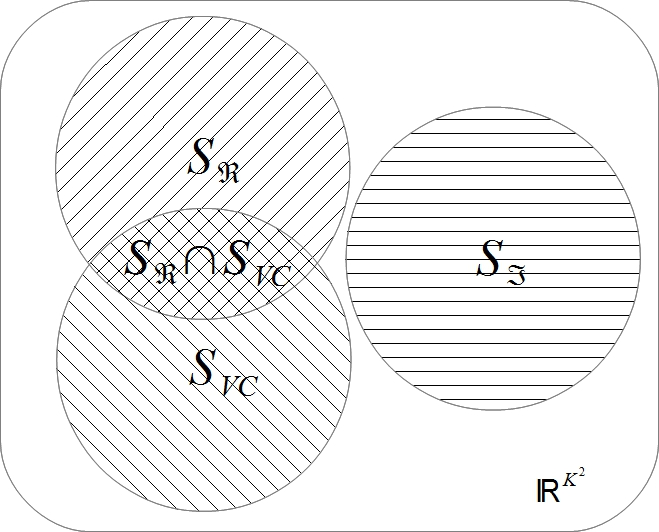
\includegraphics[width=12cm]{./images/SetsReImVC.jpg}
\caption{Взаимосвязь подпространств для кросс-спектра на уровне сенсоров}
\medskip
\small
Подпространство объемной проводимости $S_{SL}$ и подпространство действительной части кросс-спектра $S_{\Re}$
имеют непустое пересечение. Кроме того, оба этих подпространства ортогональны подпространству мнимой
части кросс-спектра $S_{\Im}$.
Пересечение $S_{SL}$ с $S_{\Re}$ содержит вклад как от протечки сигнала,
так и от истинно взаимодействующих источников,
расположенных близко друг к другу и характеризующихся малой разностью фаз.
\label{fig:subspaces}
\end{figure}%
Имея в виду все вышеперечисленное, вернемся к построению проектора.
Рассмотрим матрицу, составленную из вектор-столбцов, образующих подпространство протечки сигнала:

\begin{equation}
    \mathbf{F} = 
    \begin{bmatrix}
        |                                 & |                                 &       & |                                 \\
        \mathbf{g}_1 \otimes \mathbf{g}_1 & \mathbf{g}_2 \otimes \mathbf{g}_2 & \dots & \mathbf{g}_n \otimes \mathbf{g}_n \\
        |                                 & |                                 &       & | 
    \end{bmatrix}
\end{equation} 

Произведем сингулярное разложение матрицы $\mathbf{F}$ \cite{Golub1996}.

\begin{equation}
    \mathbf{F} = \mathbf{USV}^T 
    = 
    \begin{bmatrix}
        |            & |            &        & |       \\
        \mathbf{u}_1 & \mathbf{u}_2 & \dots  & \mathbf{u}_{m^2} \\  
        |            & |            &        & |
    \end{bmatrix}
    % S
    % \begin{pmatrix}
    %   \lambda_1 & 0         & \dots   & 0             & 0 & \dots & 0 \\
    %   0         & \lambda_2 & \dots   & \vdots        & 0 & \dots & 0 \\
    %   \vdots    &           & \ddots  & 0             & 0 & \dots & 0 \\
    %   0         & \dots     & \dots   & \lambda_{m^2} & 0 & \dots & 0
    % \end{pmatrix}
    \begin{pmatrix}
        \lambda_1 & 0         & \dots    \\
        0         & \lambda_2 & \dots    \\
        \vdots    &           & \ddots   
    \end{pmatrix}
    % Diag(\lambda_1, \dots, \lambda_{m^2})
    \begin{bmatrix}
        - & \mathbf{v}_1 & - \\
        - & \mathbf{v}_2 & - \\
          & \dots        &   \\
        - & \mathbf{v}_n & -   
    \end{bmatrix}
\end{equation}
\\
В соответствии со своиствами сингулярного разложения, первые $r$ колонок матрицы $\mathbf{U}$
образуют ортонормальный базис $r$-мерного линейного, являющегоося лучшим $r$-мерным приближением $n$-мерного
подпространства протечки сигнала. Используем эти $r$ векторов для построения проектора с уменьшенным рангом:

\begin{gather}
    \mathbf{U}_r = 
    \begin{bmatrix}
        |            & |            &        & |       \\
        \mathbf{u}_1 & \mathbf{u}_2 & \dots  & \mathbf{u}_r \\
        |            & |            &        & |
    \end{bmatrix};\\
    \mathbf{P}_r = \mathbf{I} - \mathbf{U}_r \mathbf{U}_r^T
 \end{gather} 
Итак, мы построили оператор проекции ортогонально подпространству протечки сигнала $\mathbf{P}_r$
с сокращенным рангом $r$.
Умножение уравнения (\ref{cp_rhs_kron}) на этот оператор приводит к тому, что  из порождающей
модели кросс-спектра на уровне сенсоров частично удаляются члены ответственные за эффект протечки сигнала;
параметр $r$ при этом определяет баланс между желаемым уровнем очистки от протечки сигнала и
воздействием проектора на действительную часть кросс-спектра.
Окончательно, выражение для кросс-спектра на уровне сенсоров после проекции от протечки сигнала
запишется в виде:

\begin{equation}    
    vec(\Cp{x})^\perp = \mathbf{P}_r vec(\Cp{x}) =  \sum\limits_{p=1}^n\sum\limits_{q=1}^n \mathbf{P}_r \mathbf{g}_q\otimes \mathbf{g}_p \cdot c_{pq}^{\mathbf{ss}}(t) + \mathbf{P}_r vec(\Cp{\omega}(t))
    \label{cp_final}
\end{equation}  

Элементы полученного таким образом векторизованного кросс-спектра $vec(\Cp{x})^\perp$ теперь могут быть использованы для изучения коннективностей в мозге как на уровне сенсоров, так и в источниках.

\subsection{Модели со свободной ориентацией диполя}
С точки зрения анатомии каждая топография прямой модели $\mathbf{G}$
представляет собой распределение электромагнитного поля,
порождаемого так называемыми первичными токами, то есть токами,
текущими через апикальные дендриты кортикальных пирамидальных нейронов.
Так как апикальные дендриты расположены перпендикулярно к кортикальной мантии,
первичные токи по отношению к кортикальной мантии также имеют нормальную ориентацию.
Следовательно, точность прямой модели напрямую зависит от точности оценки вектора нормали
к поверхности коры, а значит и от количества точек, используемых для аппроксимации поверхности коры.
Вместе с тем, хотя современное моделирование с использованием метода магнитно-резонансной
томографии позволяет получать весьма детальную реконструкцию мозга с размером аппроксимирующих сеток 
порядка нескольких сотен тысяч узлов, использование столь подробных сеток приводит к значительному
ухудшению производительности алгоритмов, работающих в пространстве источников, вследствие высоких затрат
по памяти и вычислительному времени при работе с большими массивами данных.

По этой причине использование разреженных сеток со сравнительно небольшим числом узлов является
общепринятой практикой.

Эту процедуру следует выполнять осторожно, так как разрежение приводит к потере информации о направлениях ориентаций нормалей. Неопределенность исходит из того, что после разрежения узлы сетки будут представлять собой пространственные пятна на кортикальной поверхности с разными степенями кривизны. Изменение местоположения активации внутри отдельного пятна приводит к сдвигу нормали и соответствующей топографии. Общий подход к оценке данного эффекта заключается в том, чтобы выделить нормаль к каждому пятну, имеющую свободную ориентацию, с помощью введения дополнительных параметров в модель [13].
Для того чтобы это сделать, следует представить топографию в месте p в виде линейной комбинации трех ортогональных друг к другу векторов топографии, размещенных в одной точке, следующим образом:

27
В случае, если измерения проводятся с помощью МЭГ, с того момента как создаваемое диполем с радиальной ориентацией магнитное поле, находящееся вне сферического проводника, равно нулю, введенная тройка векторов может быть перемещена парой диполей в локальную касательную плоскость, рассчитываемую для каждого узла. Следовательно, уравнение МЭГ (27) перепишется в виде

28
Соответственно, мы должны изменить выражение и для топографии объемной проводимости:

29
Таким образом, мы видим, что 2-топографии объемной проводимости теперь представлены тройками векторов, а именно Результирующая 2-топография объемной проводимости зависит только от параметра  и угла между направлением топографии и ее х-компоненты и, таким образом, и результирующий вектор запишется в виде
Но это 1-параметрическое семейство не может быть приведено к линейному пространству с размерностью меньше 3, чтобы проецировать из него. Значит, мы должны добавить все 3 2-топографии источника р в матрицу F для построения проектора:
%\newpage
%============================================================================================================================

\section{Ссылки} \label{sect1_2}
Сошлёмся на библиографию.
Одна ссылка: \cite[с.~54]{Sokolov}\cite[с.~36]{Gaidaenko}.
Две ссылки: \cite{Sokolov,Gaidaenko}.
Много ссылок: %\cite[с.~54]{Lermontov,Management,Borozda} % такой «фокус» вызывает biblatex warning относительно опции sortcites, потому что неясно, к какому источнику относится уточнение о страницах, а bibtex об этой проблеме даже не предупреждает
\cite{Lermontov,Management,Borozda,Marketing,Constitution,FamilyCode,Gost.7.0.53,Razumovski,Lagkueva,Pokrovski,Sirotko,Lukina,Methodology,Encyclopedia,Nasirova,Berestova,Kriger}.
И~ещё немного ссылок:
\cite{Article,Book,Booklet,Conference,Inbook,Incollection,Manual,Mastersthesis,Misc,Phdthesis,Proceedings,Techreport,Unpublished}.
\cite{medvedev2006jelektronnye, CEAT:CEAT581, doi:10.1080/01932691.2010.513279,Gosele1999161,Li2007StressAnalysis, Shoji199895,test:eisner-sample,AB_patent_Pomerantz_1968,iofis_patent1960}

%Попытка реализовать несколько ссылок на конкретные страницы для стандартной реализации:[\citenum{Sokolov}, с.~54; \citenum{Gaidaenko}, с.~36].

%Несколько источников мультицитата (только в biblatex)
%\cites[vii--x, 5, 7]{Sokolov}[v"--~x, 25, 526]{Gaidaenko} поехали дальше

Ссылки на собственные работы:~\cite{vakbib1, confbib1}

Сошлёмся на приложения: Приложение \ref{AppendixA}, Приложение \ref{AppendixB2}.

Сошлёмся на формулу: формула \eqref{eq:equation1}.

Сошлёмся на изображение: рисунок \ref{img:knuth}.

%\newpage
%============================================================================================================================

\section{Формулы} \label{sect1_3}

Благодаря пакету \textit{icomma}, \LaTeX~одинаково хорошо воспринимает в качестве десятичного разделителя и запятую ($3,1415$), и точку ($3.1415$).

\subsection{Ненумерованные одиночные формулы} \label{subsect1_3_1}

Вот так может выглядеть формула, которую необходимо вставить в строку по тексту: $x \approx \sin x$ при $x \to 0$.

А вот так выглядит ненумерованая отдельностоящая формула c подстрочными и надстрочными индексами:
\[
(x_1+x_2)^2 = x_1^2 + 2 x_1 x_2 + x_2^2
\]

При использовании дробей формулы могут получаться очень высокие:
\[
  \frac{1}{\sqrt{2}+
  \displaystyle\frac{1}{\sqrt{2}+
  \displaystyle\frac{1}{\sqrt{2}+\cdots}}}
\]

В формулах можно использовать греческие буквы:
\[
\alpha\beta\gamma\delta\epsilon\varepsilon\zeta\eta\theta\vartheta\iota\kappa\lambda\\mu\nu\xi\pi\varpi\rho\varrho\sigma\varsigma\tau\upsilon\phi\varphi\chi\psi\omega\Gamma\Delta\Theta\Lambda\Xi\Pi\Sigma\Upsilon\Phi\Psi\Omega
\]

\def\slantfrac#1#2{ \hspace{3pt}\!^{#1}\!\!\hspace{1pt}/
  \hspace{2pt}\!\!_{#2}\!\hspace{3pt}
} %Макрос для красивых дробей в строчку (например, 1/2)
Для красивых дробей (например, в индексах) можно добавить макрос
\verb+\slantfrac+ и писать $\slantfrac{1}{2}$ вместо $1/2$.
%\newpage
%============================================================================================================================

\subsection{Ненумерованные многострочные формулы} \label{subsect1_3_2}

Вот так можно написать две формулы, не нумеруя их, чтобы знаки равно были строго друг под другом:
\begin{align}
  f_W & =  \min \left( 1, \max \left( 0, \frac{W_{soil} / W_{max}}{W_{crit}} \right)  \right), \nonumber \\
  f_T & =  \min \left( 1, \max \left( 0, \frac{T_s / T_{melt}}{T_{crit}} \right)  \right), \nonumber
\end{align}

Выровнять систему ещё и по переменной $ x $ можно, используя окружение \verb|alignedat| из пакета \verb|amsmath|. Вот так: 
\[
    |x| = \left\{
    \begin{alignedat}{2}
        &&x, \quad &\text{eсли } x\geqslant 0 \\
        &-&x, \quad & \text{eсли } x<0
    \end{alignedat}
    \right.
\]
Здесь первый амперсанд (в исходном \LaTeX\ описании формулы) означает выравнивание по~левому краю, второй "--- по~$ x $, а~третий "--- по~слову <<если>>. Команда \verb|\quad| делает большой горизонтальный пробел.

Ещё вариант:
\[
    |x|=
    \begin{cases}
    \phantom{-}x, \text{если } x \geqslant 0 \\
    -x, \text{если } x<0
    \end{cases}
\]

Кроме того, для  нумерованых формул \verb|alignedat|  делает вертикальное
выравнивание номера формулы по центру формулы. Например,  выравнивание компонент вектора:
\begin{equation}
 \label{eq:2p3}
 \begin{alignedat}{2}
{\mathbf{N}}_{o1n}^{(j)} = \,{\sin} \phi\,n\!\left(n+1\right)
         {\sin}\theta\,
         \pi_n\!\left({\cos} \theta\right)
         \frac{
               z_n^{(j)}\!\left( \rho \right)
              }{\rho}\,
           &{\boldsymbol{\hat{\mathrm e}}}_{r}\,+   \\
+\,
{\sin} \phi\,
         \tau_n\!\left({\cos} \theta\right)
         \frac{
            \left[\rho z_n^{(j)}\!\left( \rho \right)\right]^{\prime}
              }{\rho}\,
            &{\boldsymbol{\hat{\mathrm e}}}_{\theta}\,+   \\
+\,
{\cos} \phi\,
         \pi_n\!\left({\cos} \theta\right)
         \frac{
            \left[\rho z_n^{(j)}\!\left( \rho \right)\right]^{\prime}
              }{\rho}\,
            &{\boldsymbol{\hat{\mathrm e}}}_{\phi}\:.
\end{alignedat}
\end{equation}

Ещё об отступах. Иногда для лучшей <<читаемости>> формул полезно
немного исправить стандартные интервалы \LaTeX\ с учётом логической
структуры самой формулы. Например в формуле~\ref{eq:2p3} добавлен
небольшой отступ \verb+\,+ между основными сомножителями, ниже
результат применения всех вариантов отступа:
\begin{align*}
\backslash! &\quad f(x) = x^2\! +3x\! +2 \\
  \mbox{по-умолчанию} &\quad f(x) = x^2+3x+2 \\
\backslash, &\quad f(x) = x^2\, +3x\, +2 \\
\backslash{:} &\quad f(x) = x^2\: +3x\: +2 \\
\backslash; &\quad f(x) = x^2\; +3x\; +2 \\
\backslash \mbox{space} &\quad f(x) = x^2\ +3x\ +2 \\
\backslash \mbox{quad} &\quad f(x) = x^2\quad +3x\quad +2 \\
\backslash \mbox{qquad} &\quad f(x) = x^2\qquad +3x\qquad +2
\end{align*}


Можно использовать разные математические алфавиты:
\begin{align}
\mathcal{ABCDEFGHIJKLMNOPQRSTUVWXYZ} \nonumber \\
\mathfrak{ABCDEFGHIJKLMNOPQRSTUVWXYZ} \nonumber \\
\mathbb{ABCDEFGHIJKLMNOPQRSTUVWXYZ} \nonumber
\end{align}

Посмотрим на систему уравнений на примере аттрактора Лоренца:

\[ 
\left\{
  \begin{array}{rl}
    \dot x = & \sigma (y-x) \\
    \dot y = & x (r - z) - y \\
    \dot z = & xy - bz
  \end{array}
\right.
\]

А для вёрстки матриц удобно использовать многоточия:
\[ 
\left(
  \begin{array}{ccc}
    a_{11} & \ldots & a_{1n} \\
    \vdots & \ddots & \vdots \\
    a_{n1} & \ldots & a_{nn} \\
  \end{array}
\right)
\]


%\newpage
%============================================================================================================================
\subsection{Нумерованные формулы} \label{subsect1_3_3}

А вот так пишется нумерованая формула:
\begin{equation}
  \label{eq:equation1}
  e = \lim_{n \to \infty} \left( 1+\frac{1}{n} \right) ^n
\end{equation}

Нумерованых формул может быть несколько:
\begin{equation}
  \label{eq:equation2}
  \lim_{n \to \infty} \sum_{k=1}^n \frac{1}{k^2} = \frac{\pi^2}{6}
\end{equation}

Впоследствии на формулы (\ref{eq:equation1}) и (\ref{eq:equation2}) можно ссылаться.

Сделать так, чтобы номер формулы стоял напротив средней строки, можно, используя окружение \verb|multlined| (пакет \verb|mathtools|) вместо \verb|multline| внутри окружения \verb|equation|. Вот так:
\begin{equation} % \tag{S} % tag - вписывает свой текст 
  \label{eq:equation3}
    \begin{multlined}
        1+ 2+3+4+5+6+7+\dots + \\ 
        + 50+51+52+53+54+55+56+57 + \dots + \\ 
        + 96+97+98+99+100=5050 
    \end{multlined}
\end{equation}

Используя команду \verb|\labelcref| из пакета \verb|cleveref|, можно
красиво ссылаться сразу на несколько формул
(\labelcref{eq:equation1,eq:equation3,eq:equation2}), даже перепутав
порядок ссылок \verb|(\labelcref{eq:equation1,eq:equation3,eq:equation2})|.

